\subsection{Methodology}
\subsubsection{Data Collection}
In the beginning our idea was to automate the data collection by using OpenWPM, a tool that automates the tasks of controlling a browser and collecting data. However, after some time it turned out that the general effort to set up such automation is not proportionate to the data we ultimately need. The only advantage would have been to replicate the user journey one-to-one and then possibly have more consistent data available. Nevertheless, we are now continuing with the manual data collection approach.

To analyze the cross-device tracking capabilities of various news websites, we conducted a systematic data collection using HTTP Archive (HAR) files. This process involved capturing network traffic data from both desktop and mobile devices. We selected our set of 20 websites by first categorizing them into news websites and shopping websites. These websites were chosen based on their popularity and the diversity of their content and geographical origin.

Prior to data collection, we created a test account on each of the selected websites. This was essential to ensure consistency in the user experience and to capture potential deterministic cross device tracking data across different sessions and devices.

To standardize the browsing environment and eliminate the most external variables, the data collection was executed using a virtual machine. This enables us to attribute any differences observed in the tracking mechanisms to the device type rather than other environmental factors.

Google Chrome was used as the web browser for this exercise as its developer tools with many functionalities allowed us to generate the HAR files. 

The first part of the data collection involved accessing each news website from a desktop device. The user journey for all websites of both categories started with logging in using the previously created test account. For news websites the second part was navigating to a prominent news topic and try to imitate common user behavior. For shopping websites the second part included adding one or more items to the shopping cart and then proceed to checkout, but stop just before the actual payment. 

The same procedure was replicated on mobile devices, to be more precise on an iPhone, in order capture the mobile user experience on the same websites. The HAR files of the mobile user journey was captured using Safari Developer Tools while connecting the iPhone to the MacBook via cable.

The resulting data set comprised 40 HAR files - 10 from desktop devices and 10 from mobile devices, corresponding to the same set of news websites and shopping websites. This data set will be the starting point for our subsequent analysis of cross-device tracking practices.
\subsubsection{Data Analysis}

\begin{figure}[ht]
    \centering
    \begin{subtable}[b]{0.3\textwidth}
        \centering
        \begin{tabular}{|l|l|}
            \hline
            \multicolumn{2}{|c|}{\textbf{cookieLog}} \\
            \hline
            id           & INT \\
            domain       & TEXT \\
            host         & TEXT \\
            device\_type  & TEXT \\
            website\_type & TEXT \\
            \hline
        \end{tabular}
        \caption{cookieLog}
    \end{subtable}
    \hfill
    % Table 2: emailHashes
    \begin{subtable}[b]{0.3\textwidth}
        \centering
        \begin{tabular}{|l|l|}
            \hline
            \multicolumn{2}{|c|}{\textbf{emailHashes}} \\
            \hline
            id           & INT \\
            host         & TEXT \\
            hash\_type    & TEXT \\
            domain       & TEXT \\
            device\_type  & TEXT \\
            website\_type & TEXT \\
            \hline
        \end{tabular}
        \caption{emailHashes}
    \end{subtable}
    \hfill
    \begin{subtable}[b]{0.3\textwidth}
        \centering
        \begin{tabular}{|l|l|}
            \hline
            \multicolumn{2}{|c|}{\textbf{thirdPartyLog}} \\
            \hline
            id           & INT \\
            domain       & TEXT \\
            host         & TEXT \\
            device\_type  & TEXT \\
            website\_type & TEXT \\
            \hline
        \end{tabular}
        \caption{thirdPartyLog}
    \end{subtable}
\end{figure}
Since our data is relatively large (50-100MB per HTTP archive), we performed most of the analysis using Jupyter Notebooks and the Python library haralyzer. In the initial stages of our data analysis, we began with a traditional approach, using print statements to inspect and debug the data. This method, while straightforward, quickly proved to be inadequate for handling larger datasets. As the volume and complexity of the data increased, it became apparent that a more robust and scalable solution was necessary. We then started to set up a database that includes three tables in the following way, so we can perform the major part of our analysis with a small delay using simple SQL statements in combination with python scripts. The query results were then visualized using diagrams.

Our approach was then to determine which parts of the HTTP requests are relevant for us to make statements about cross-device tracking activities.

The first and perhaps most important part of our analysis consisted of filtering out HTTP requests that were sent to third-party domains. We are particularly interested in which domain the request was sent to and how often requests to such domains were recorded. We also wanted to compare the websites with each other in terms of the number of requests to third-party providers. We used the thirdPartyLog table in our database to filter and visualize the respective requests.

It is also interesting to see whether any sensitive data was sent to third-party providers. This means that we examine all HTTP requests and responses to see whether a simple, hashed or encrypted version of our email address can be found. We looked for plain and base64 encoded versions of our mail address as well as SHA1, SHA256, SHA224 and SHA512. In order filter and visualize our results, we used the emailHashes table of our database.

To get a general overview of the cookies set, we also wanted to determine the specific domains that have set the most cookies and possibly establish a correlation with the third-party domains that were requested the most. We focused on the quantity of cookies set by each domain, offering insight into the role these entities play in the broader context of online tracking, particularly in cross-device scenarios. We used the cookieLog table for this part.

In order to also qualitatively analyze the cookies that were set, we looked at each website to see if there were identical cookies that were set for the same website on the desktop and the mobile device. To be even more specific, we checked which cookies could be identifiers that are used to uniquely identify a user across multiple devices so that, for example, customized advertising can be placed. This part is done manually as we have to look at possible identifiers by ourselves, because it is difficult to automatically filter out identifiers.

In the last part of our analysis, we wanted to carry out a comparative analysis. In fact, we have two variables that seem interesting for comparison. First, the device type, to show differences in behavior between mobile and desktop devices, and second, the website category by which we divided our websites in the initial step.

Our plan was to conduct the previous analysis again, but this time to differentiate and look at the relevant category. In the best case scenario, we can see interesting results that give an indication of which categories are more affected by cross device tracking activities.

\subsection{Results}
\subsubsection{Requests to third party domains}
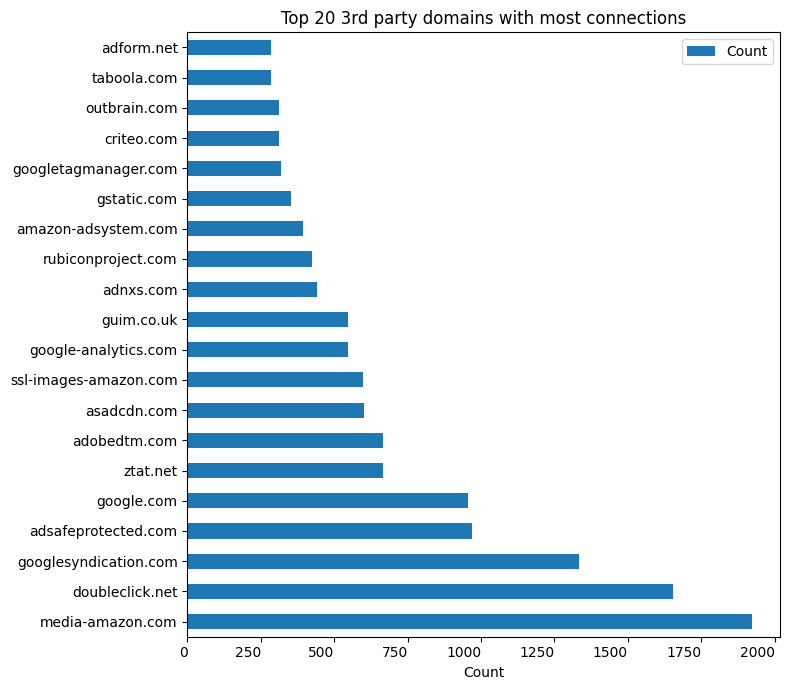
\includegraphics[width=0.8\textwidth]{./assets/top20thirdpartydomains.png}

In our test runs on news and shopping sites, we were able to identify links to a total of 537 different third-party domains. Some of the domains were operated by the website that we observed. For example theguardian.com connected to guardianapps.co.uk which is obviously operated by the same company and is no third party. We tried to filter out the majority of all domains that belong to the same company as the website we were observing, but it is possible, that we missed some. Additionally, it was noticeable that most of the domains we found were connected to or part of Google and Amazon (see table). But we were also able to collect queries to other major tech companies such as Microsoft, Facebook and even TikTok. 

This shows once again how big a role these companies play in the context of online user tracking. Of course, this doesn't prove cross-device tracking, but it does give us an indication of how much data is being shared with third parties, and the likelihood that this data is being used to create accurate user profiles.
\begin{table}[ht]
\small
\centering
\begin{tabularx}{0.6\textwidth}{|X|X|}
\hline
\textbf{Amazon} & \textbf{Google} \\
\hline
media-amazon.com & doubleclick.net \\
ssl-images-amazon.com & googlesyndication.com \\
amazon-adsystem.com & google.com \\
amazon.com & google-analytics.com \\
cloudfront.net & gstatic.com \\
amazonaws.com & googletagmanager.com \\
 & googletagservices.com \\
 & google.de \\
 & googleapis.com \\
 & googleadservices.com \\
 & recaptcha.net \\
 & youtube.com \\
 & ytimg.com \\
\hline
\end{tabularx}
\caption{third-party domains related to Amazon and Google}
\label{tab:third-party-domains}
\end{table}

\vspace{0.5cm}
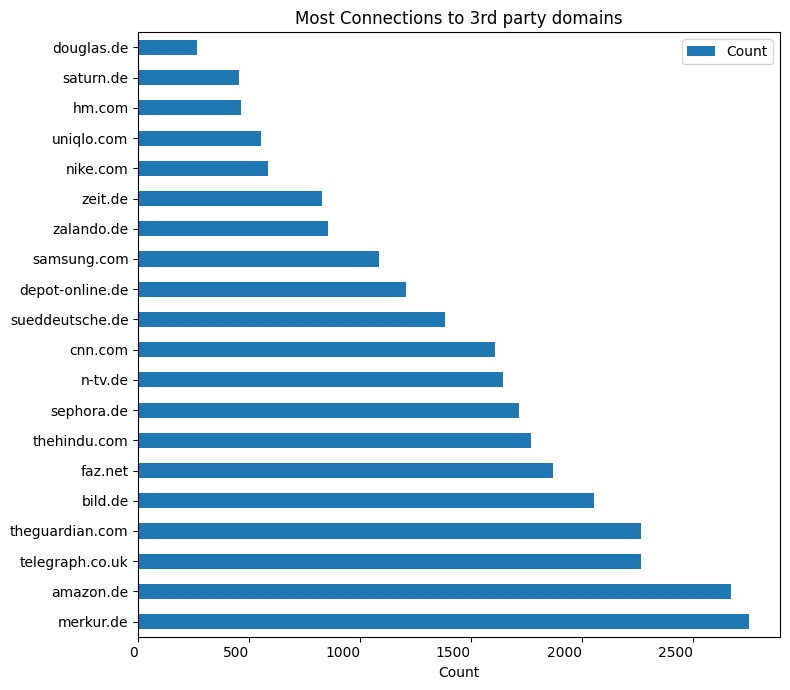
\includegraphics[width=0.8\textwidth]{./assets/mostConnectionsToThirdPartyDomains.png}
\vspace{0.5cm}

We observed that more than half of all websites have made more than 1000 requests to third party domains. Four websites even made more than 2000 requests. 

The bar chart illustrates the diversity of third-party domain connections by showing the number of unique domains to which each site communicated. On average, a website made 1,416 requests to approximately 72 different third-party domains. This is typical of the complex network of third party services that modern sites rely on.

A notable exception case is Amazon, which had the second highest total number of requests but interacted with only 17 unique domains. This anomaly could indicate a reliance on a select set of services, possibly indicating Amazons strategy of using proprietary systems for cross-device tracking and other functions, thereby limiting interactions with external third parties. Such a strategy could reflect enhanced data control measures and a consolidated approach to digital tracking.

\subsubsection{Sensitive Information to third party providers}
In the study of sensitive information sharing with third parties, particularly focusing on email data, both hashed and plain, significant insights were revealed. The analysis centered on tracking the flow of email addresses to various third-party websites. The findings indicate a diverse range of websites receiving this sensitive data, with notable variations in the frequency and method of information sharing.

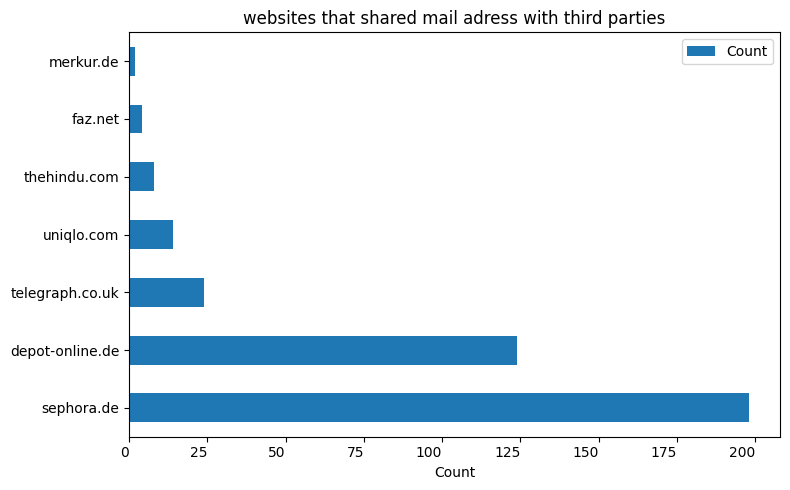
\includegraphics[width=0.8\textwidth]{./assets/websitesSharingMailAddresses.png}

Moreover, when analyzing the encryption methods used, a predominant reliance on SHA256 hashing is observed. This pattern suggests a general preference for SHA256 as a security measure in the transfer of email data. However, instances of plain text email sharing are not absent, as evidenced by c2.piano.io and news.google.com, which shared email addresses 8 and 7 times, respectively, without encryption.

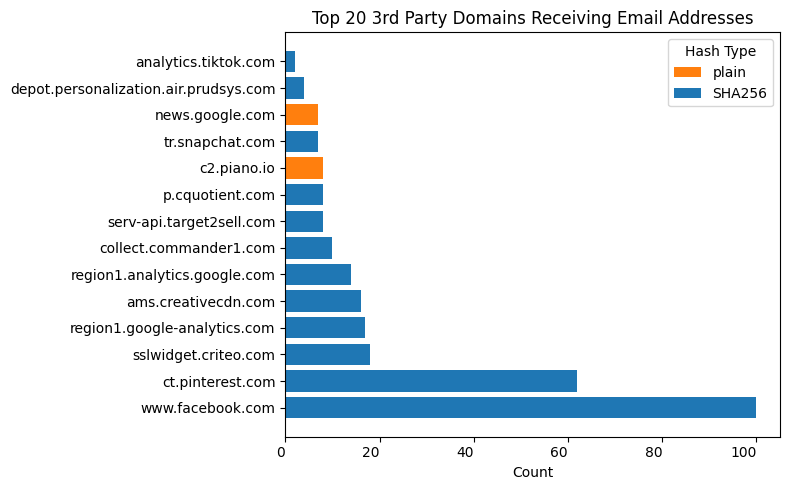
\includegraphics[width=0.8\textwidth]{./assets/top20thirdpartydomainsreceivingmailaddresses.png}

It should be noted that almost half of all email address transfers were initiated by Sephora. The sensitive data was in turn shared with big tech companies such as Facebook, Google and surprisingly even Snapchat and TikTok.

These findings raise critical discussions about the privacy and security measures in place for the transfer of sensitive data like email addresses. The varied use of encryption methods, along with the sheer number of third parties involved, highlights the complexity and potential vulnerabilities in the current digital landscape regarding data privacy.


\subsubsection{Cookie Analysis}
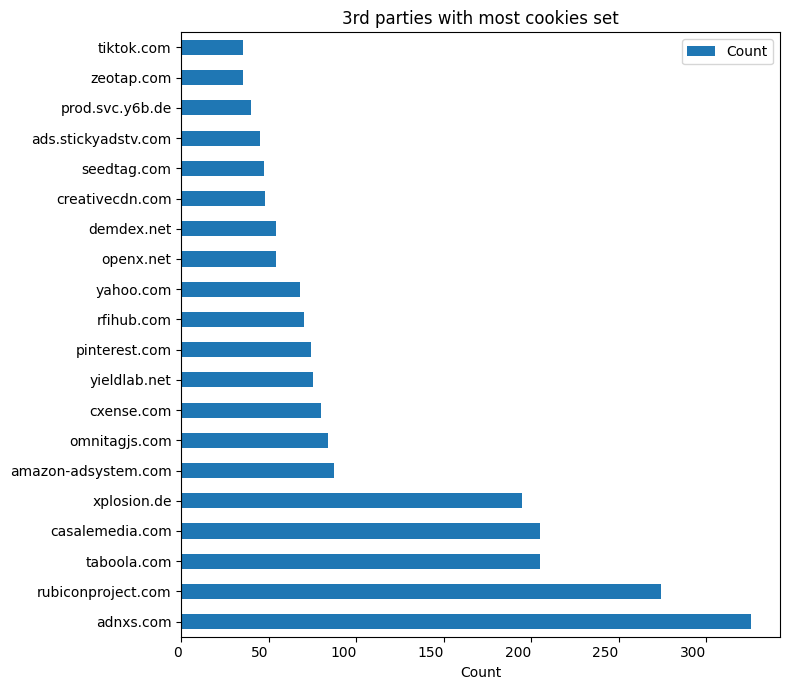
\includegraphics[width=0.8\textwidth]{./assets/thirdpartieswithmostcookiesset.png}

Certain domains, such as adnxs.com (AppNexus), taboola.com and rubiconproject.com showed a high frequency in cookies set and amount of connections from our test websites and were leading in terms of the number of requests, which indicates their comprehensive role in tracking and advertising across multiple platforms.

This underscores their significant role in the digital advertising ecosystem, especially in cross-device tracking. Amazon, through domains like amazon-adsystem.com and Google through domains like youtube.com, emerged as prominent trackers as well, but surprisingly despite having registered a high number of connections from our test websites, were much less dominant in cookie setting in comparison to the previously mentioned competing providers. 

This finding suggests, that the big players are more likely to use alternative tracking mechanisms beyond traditional cookies, possibly including fingerprinting or pixel tracking.This finding aligns with its vast online presence and interest in user data for both e-commerce and advertising purposes.

The high volume of cookies set by these entities in genereal suggests an extensive network of data collection, crucial for building comprehensive user profiles across different devices.


\subsubsection{Duplicate identifiers across mibile and desktop devices}
As we have logged in in the beginning of all our test runs, it is likely that the websites have cross device tracked the test user via deterministic cross device tracking. Our analysis revealed several cookies with equal values across devices, indicating their potential use as cross-device identifiers. The relevant output can be found in appendix 1 and include:
\begin{enumerate}
    \item DSID and User IDs: Various user ID cookies, were consistently found across devices. For instance, userId in faz.net and authId in sueddeutsche.de, with their unique alphanumeric strings, suggest a potential for user-specific identification across different browsing sessions and devices.
    \item Encoded and Hashed Values: Cookies with base64 encoded strings (e.g., u in cnn.com) or hash values (e.g., hasheduseremail in sephora.de) were identified as consistent across devices. These formats are typically used to encode identifiable information in a non-readable format, enhancing security while still allowing for user tracking.
    \item Unique Device or Session Identifiers: Cookies like UUID in merkur.de, with values that seem to be unique to each user, appeared consistently across different devices. This uniqueness is a strong indicator of their role in cross-device identification.
\end{enumerate}
The presence of equal identifiers across devices underscores the sophisticated nature of current online tracking methodologies. These identifiers enable a seamless tracking experience, allowing advertisers and websites to create comprehensive user profiles by linking activities across multiple devices. This capability has significant implications for targeted advertising and personalized content delivery.

The results suggest that once websites have established a user's identity using deterministic methods, as indicated by cookies such as userId and authId, the next step is often cookie synchronisation. This process involves passing unique identifiers to third parties who can then use them to match the user's profile in their own databases. For example, the consistent appearance of UUID cookies across devices provides a solid foundation for synchronisation processes. The transfer of such cookies to different domains, as evidenced by the breadth of cookie syncing in our data, implies a sophisticated network where user information is exchanged to allocate a user to one or more devices.

The implications of cookie syncing are magnified when considered in the context of graph sharing. By piecing together data points from multiple sources, companies create comprehensive graphs that map a user's digital footprint across multiple devices. These graphs are not static; they are dynamic, evolving with each user interaction and feeding into algorithms that refine the understanding of user behaviour.

Given that identifiers such as DSID and hashed values such as hasheduseremail are consistent across devices, the likelihood of these being used to create cross-device graphs is high. The entities that receive these synchronised cookie values, such as third party advertising technology domains, are willing to construct or contribute to the construction of these graphs.